\documentclass[titlepage]{article}
\title{EE677 Course Project\\[1cm]\textbf{epsilon-to-verilog} : An Educational Hardware Compiler\\[1cm]}
\addtolength{\textwidth}{2in}
\addtolength{\hoffset}{-1in}
\usepackage{hyperref}
\usepackage{graphicx}
\author{Anaykumar Joshi\\
        \texttt{anaykumar.joshi@gmail.com}\\
        \texttt{Roll No. 09007019}
        \and Savant Krishna\\
        \texttt{savant.2020@gmail.com}\\
        \texttt{Roll No. 100070056}
        }
\begin{document}
\maketitle
\tableofcontents

\section{Introduction and Motivation}
        \textbf{epsilon} is a custom minimalistic language developed to create an educational platform for high level synthesis. This document introduces epsilon and explains the implementation of a verilog backend for epsilon. This doc also explains how to create a new backend (for epsilon) from scratch and the future improvements that are possible in this tool (epsilon-to-verilog). The Verilog backend implemented is a minimalistic one with each instruction of the control flow graph (cfg) considered as a state.


    The Epsilon framework is primarily intended to provide a simple platform for students to implement and test HLS algorithms.
    Present open-source High Level Synthesis compilers (example: \href{http://legup.eecg.utoronto.ca}{legup}, \href{http://c-to-verilog.com}{c-to-verilog}) typically use the \textbf{LLVM} compiler framework (Low Level Virtual Machine). For students who wish to study HLS algorithms and play around with a simple hardware compiler, LLVM can be a major stumbling block. Epsilon has tried to fill in the gap for a simple, clean, minimalistic interface for jumping into HLS!
    
\section{The Epsilon Framework}
    Epsilon has been implemented entirely in \texttt{Python-2.7}. This allows a quick and dirty prototype of a hardware compiler
    Note that the framework itself should be (literally) written as "Epsilon" (capital E), and the language in the framework should be written as "epsilon" (small e).\\
    The Epsilon framework contains three components
    \begin{itemize}
    \item A compiler
    \item A simulator
    \item An interface to Control Flow Graph (to write a backend)
    \end{itemize}
\subsection{The epsilon Language}
    epsilon is an over-simplified language. A program written in epsilon contains a single function with any number of inputs
    and any number of outputs. Every instruction is either a two-variable or three-variable instruction.
    For conditional jumping, \texttt{if} ,  \texttt{if-else} and \texttt{while} loops are provided. The scope of every variable is the entire function body.
    The language is so simple, that having a look at a few example programs written in epsilon should be enough for you to start writing
    programs in epsilon! Do have a look at \textsf{``.../examples/''} folder for example programs written in epsilon.

    One feature of the epsilon language which is not obvious is that of  ``summary''. Every epsilon function contains a summary of that function which is specified in the function body contained within two hashes.
    Here is a program written in epsilon which calculates the sum of first ``N'' numbers:
    \begin{verbatim}
        function(N) {
            
        # this function calculates the sum of first n numbers #
            i = 0
            sum = 0
            c = 1
            while (c) {
                sum = sum + i
                i = i+1
                if(i>=N) {
                    c = 0
                }
            }
            
            return(sum)
        }
    \end{verbatim}
    
    \subsection{The Epsilon Simulator}
    \label{simulator}
    The epsilon language can actually be used as a stand-alone language for general computation (though you would latter regret
    the decision of using epsilon as a general purpose langage!). So why do we have a simulator in the Epsilon framework?


    Suppose you wish to write a compiler to convert programs written in the epsilon language into a corressponding 
    synthesizeable verilog code. You would need to write a backend using the Epsilon framework \ref{backend}. Assuming that you have 
    written a backend, you would need to test your backend on some examples. Say you write a program (in the epsilon language) 
    to calculate
    the sum of first N numbers (as shown above). Before synthesizing this code to the verilog backend, it would be neat if you could simulate the program
    in the epsilon simulator to verify the correctness of the program. ie, the program written in the epsilon language is working the way you intend it should (to avoid pulling your hair latter on when the synthesized verilog code is not giving the output you expect!)


    To simulate a program written in epsilon language, call the \texttt{run\_simulator} method on the epsilon instance. You would be
    presented with a shell. Type "help" for a list of functions provided. 
    \begin{itemize}
    \item \texttt{summary} : Prints out the summary string contained in the epsilon program being simualated
    \item \texttt{clear}   : Clears the screen
    \item \texttt{exit}    : exits the simulator
    \item \texttt{help}    : help ?
    \end{itemize}
    To actually simulate the epsilon function, directly pass the input values separated by space. For example, if you are simulating
    a function which takes two input arguments, then simply input two values (integers) in the simulator shell separated by space.
    The result would be the vector returned by the function. (refer to screencast if you are confused)
    
    \subsection{Writing a Backend}
    \label{backend}
    Suppose you wish to write a new backend using the Epsilon framework. 
    You would need to import modules ``epsilon'' and ``epsilon\_cfg''. Create an instance of epsilon.Epsilon; let us name the instance as demo\_epsilon. You can call a few meaningful methods on demo\_epsilon now:
    \begin{itemize}
    \item \texttt{register\_backend(\emph{backend\_instance})}
    \item \texttt{run\_frontend(\emph{source\_filename.epsilon})}
    \item \texttt{run\_simulator()}
    \item \texttt{run\_backend()}
    \item \texttt{dump\_cfg()}
    \item \texttt{dump\_sim\_assembly()}
    \item \texttt{dump\_ast()}
    \end{itemize}
    PS: At present, there is a bug in \texttt{dump\_ast()} method; the generated ast dot file is not correct
    To write a new backend, create a class which inherits from \texttt{epsilon.Backend}; this backend must have a \texttt{run()} method.
    When you call \texttt{run\_backend} on the epsilon instance, the \texttt{run()} method of the last "registered" backend is called.
    To register a backend, create an instance of the backend class that you have created and call \texttt{register\_backend()} method
    on the epsilon instance with the backend instance as the argument



    \section{The Verilog backend}

    In this section, we would briefly explain the implementation of a simple verilog backend which uses the epsilon framework.

    \subsection{Implementation}
        This section explains the details of the implementation of a minimalistic Verilog backend. The control flow graph dumped by the frontend of epsilon is accessed and analyzed to create the resulting verilog files. The cfg consists of various basic blocks, each containing any number of instructions with pointers to other basic blocks (known as its children). In case a basic block does not have any child basicblocks, it is probably the last state corresponding to the return instruction.
        Every basic block object has following attributes
        \begin{verbatim}        
        number_of_instructions
        instruction_list
        condition
        condition_instr
        number_of_children
        child_true
        child_false
        child
        identity\end{verbatim} which help recognize the number of instructions and the kind of jump statements corresponding to the basic block. \texttt{condition} is the variable which is a \texttt{0} or \texttt{1} depending on the evaluation of \texttt{condition\_instr}. It is checked (if present), when all the instructions of the basic block are evaluated and if true state transits to \texttt{child\_true} else if false state transits to \texttt{child\_false} \\Each instruction in the basic block is a state (of the FSM) in itself with the basic block itself being a state (representing the jump instruction. Note that there is no instruction named "jump" in the cfg provided by the epsilon frontend. But there is sufficient insruction in the basic blocks which help us write down the jump instruction). Whenever the control jumps to a basic block, the state is changed to the state of the first instruction in the basic block. If there are no instructions in the basic block, the state is changed to that represented by the basic block itself (coressponding effectively to a jump statememt). 

        When in the  state coressponding to the final instruction of a basic block, the state transits to the state represented by the basic block. When current state corresponds to the state represented by a basic block, depending on whether the number of children of the basic block, state transition is made (conditional or unconditional). The states are numbered in the order of identity of the basic blocks, each instruction of every basic block being given a state number in the order of instructions in the list 'instruction\_list'.\\ The data flow path is as explained below. Each variable which is loaded a value in any of the instructions is allocated a 32-bit register (from the beginning to the end). These registers are multiplexed (controlled by the state diagram) so that they are updated as and when required. The operators are combinational blocks whose inputs are multiplexed according to the state to calculate the required variables.

        The module generated by epsilon-to-verilog takes in a clock, reset and gives out a outReady signal. The reset pin when low resets the state machine to the start state, which is generally the first basic block or the first instruction in the first basic block. The outReady is HIGH when the state machine reaches the final state from which there is no child (i.e, number of children = 0). It signifies that the output is ready and the function evaluation is over. It corresponds to the return statement in the epsilon program.
        A testbench is also implemented which instantiates the main module, takes the inputs from user and displays the final result after simulating the resulting verilog file.

    \subsection{Possible Improvements}
        The verilog backend is a minimalistic proof of concept implementation. It is roughly based on the architecture shown in the figure below. It can be improved using different algorithms for scheduling, resource allocation and binding. A new backend can also be created on the similar lines.
        
    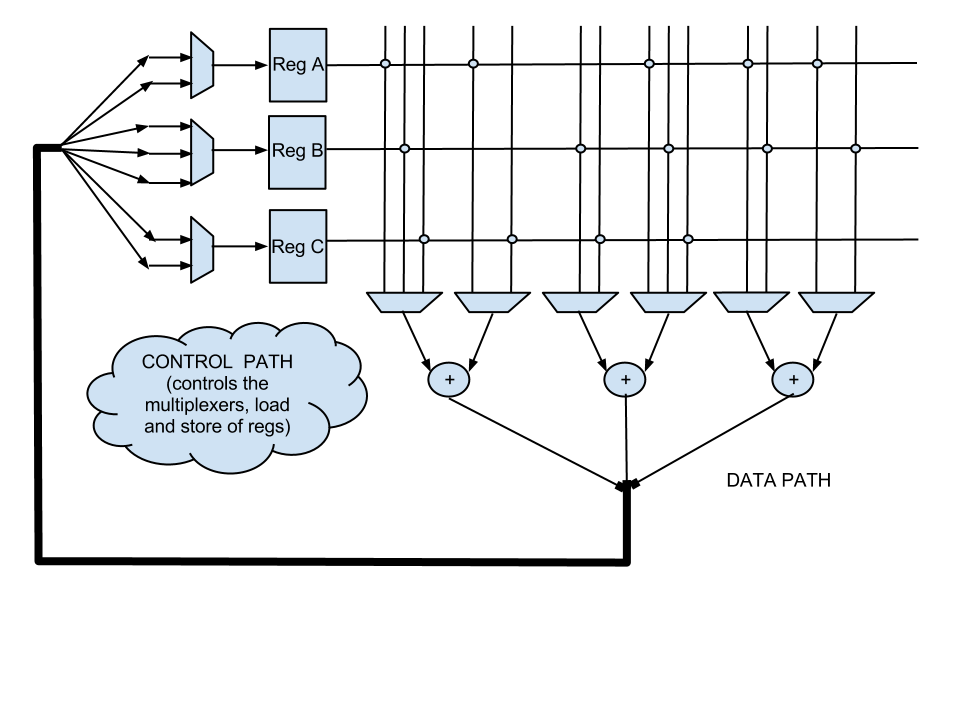
\includegraphics[scale=0.5]{architecture.png}
        
        There is almost no amount of parallelization in the current verilog backend implementation. Instructions are done sequentially and Variables are considered alive for the whole duration of the program in this implementation. One way to improve the efficiency is to schedule instructions so that independent instructions can occur simultaneously using many resources. 
        
        Another way is to have efficient memory use by determining variable liveness and reallocating registers with dead variables (variables which are not accessed in future) to other newly live variables. Variables are bound to specific registers for their lifetime, which can be figured out from the control flow graph. One more problem which should be addressed when parellizing the computation is the resource constraint. In case the hardware is resource constrained, for eg. if there can only be 3 adders possible, then suitable scheduling needs to be done to strike the balance between resources needed and the time taken for the computation.
    To make it simpler for students to work with epsilon, have a look at the screencast available with this document.

    \section{Conclusion}
    The present implementation of epsilon is quite limited, and can only be used for some
    specific architecture of hardware. Nevertheless, Epsilon should be of some use for students who are very new to HLS.
    As a suggestion, the tool epsilon-to-verilog can be used in future iterations of EE677 to introduce High Level Synthesis. 
    We would like to thank \textbf{Prof.Sachin Patkar}, \textbf{B.Y.Vinay Kumar} and \textbf{Dilawar Singh} for their motivation and constant help. Thank you :)

\end{document}

